 

\section{Resultados}\label{s:resul}

\begin{multicols}{2}

\subsection{Teste de Kruskal-Wallis}

Na Tabela \ref{tab:krusk} apresentamos o Teste de Kruskal-Wallis dos índices que analisamos. A hipótese nula $(H0)$ do teste é de que os valores de um índice específico quando agrupados pela natureza jurídica do prestador de serviços fazem parte de uma mesma população. Nota-se que somente em quatro índice rejeitamos $H0$, ou seja, para esses índices, os grupos fazem parte de populações idênticas não havendo diferenças significativas entre os prestadores de serviços.

\end{multicols}




\begin{table}[H] \centering 
\begin{minipage}{0.3\textwidth}
  \caption{Teste de Kruskal} 
  \label{tab:krusk} 
\begin{tabular}{@{\extracolsep{5pt}} ccc} 
\toprule
\toprule
Índices & \shortstack{Valor p \\ do teste} & H0 \\ 

\midrule

IN004 & $0,00$ & Rejeita \\ 
IN005 & $0,00$ & Rejeita \\ 
IN006 & $0,00$ & Rejeita \\ 
IN015 & $0,08$ & Rejeita \\ 
IN016 & $0,00$ & Rejeita \\ 
IN055 & $0,45$ & Aceita \\ 
IN012 & $0,42$ & Aceita \\ 
IN102 & $0,49$ & Aceita \\ 
IN083 & $0,06$ & Rejeita \\ 
IN008 & $0,49$ & Aceita \\ 
IN026 & $0,00$ & Rejeita \\ 

\bottomrule

\end{tabular} 
	\footnotesize \\
		Fonte: Elaborado pelos autores. 
		Nota: A hipótese nula (H0) é de que os valores dos índices são semelhantes entre as diferentes naturezas jurídicas.
\end{minipage}
\end{table} 


\begin{multicols}{2}

\subsection{Análise de correlação}

Na Figura \ref{f:corr} temos um correlograma dos índices que estamos analisando. Primeiro vamos discutir as correlações positivas e em seguida as negativas.

Nota-se que as variáveis relacionadas a tarifa média (IN004, IN005, IN006) possuem alta correlação positiva entre si, como já era de se esperar. Os índices relacionados as despesas IN008 e IN026 também possuem alta correlação positiva entre si e com os índices de despesas. Isso indica que quanto maiores as despesas, maior tende a ser as tarifas médias praticadas. 

Destaca-se também a alta correlação positiva entre o atendimento total de água (IN055) e o indicador de desempenho financeiro (IN012), isso pode ser um indicativo de que os serviços de atendimento de água são responsáveis por uma parcela significativa das receitas dos prestadores de serviços. 

Por fim, notamos também alta correlação positiva entre a despesa média anual por empregado (IN008) e o índice de produtividade (IN102). Ao que parece, maiores gastos com empregados está tendo efeito positivo na produtividade deles.

Do lado das correlações negativas temos o índice de atendimento total de água (IN055) e a despesa de exploração por m3 faturado (IN026). Aparentemente nos municípios em que a maior parte da população possui atendimento de água não é necessário investir tanto em exploração por m3 faturado.

Nota-se também alta correlação negativa entre os índices de despesa (IN008, IN026) e o indicado de desempenho financeiro (IN012). Como era de se esperar, maiores despesas diminuem os lucros e o desempenho financeiro das empresas do setor.


\end{multicols}


%--------- figure

\begin{figure}[H]
        \centering
        	\begin{minipage}{0.55\textwidth}	
                \caption{Correlograma dos índices utilizados no estudo}
                \label{f:corr}
                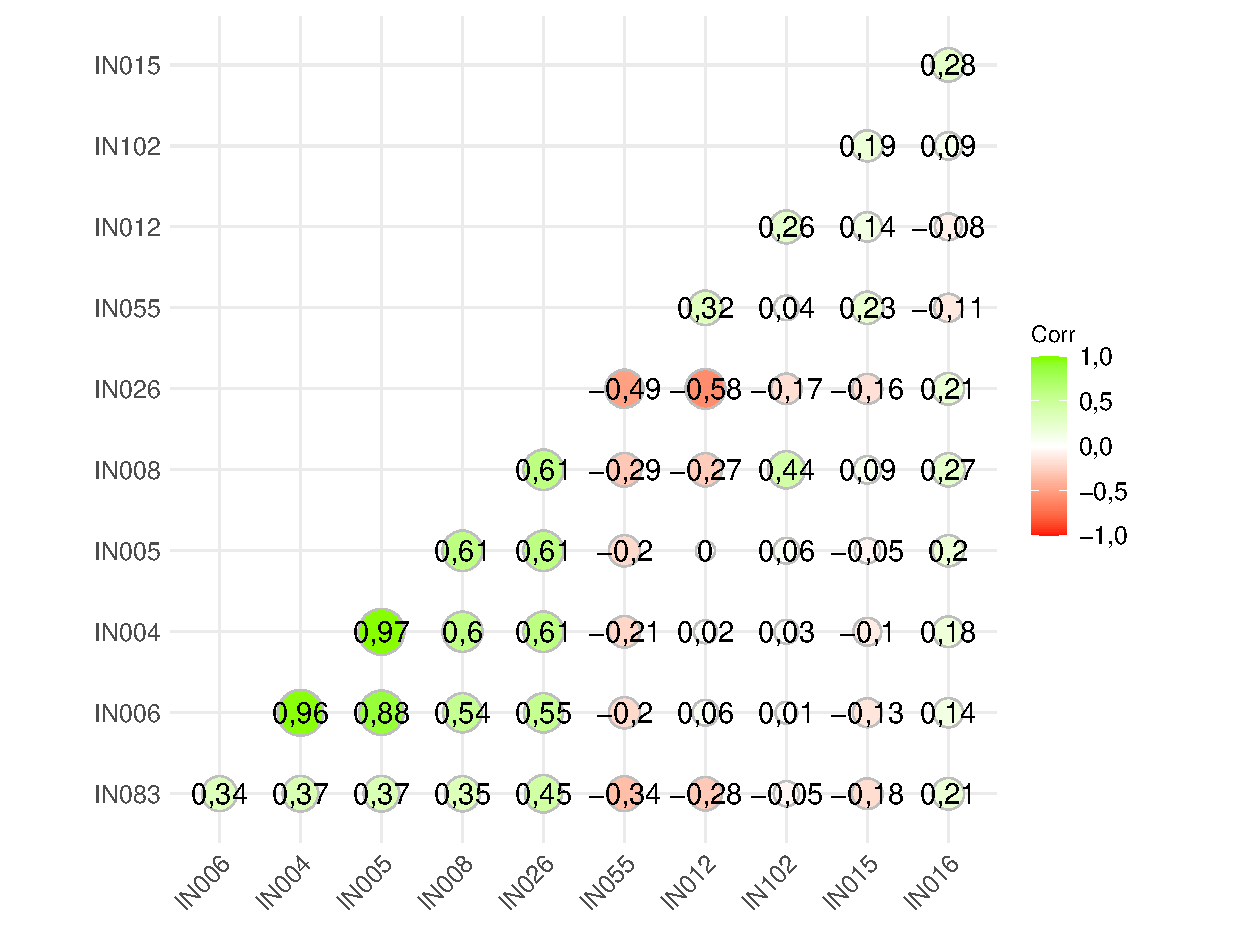
\includegraphics[scale=0.5]{figures/cor.eps}                 
            	\footnotesize \\
            		Fonte: Elaborado pelos autores com dados do SNIS. \\
            		Notas: IN004 - Tarifa média praticada,
				IN005 - Tarifa média água,
				IN006 - Tarifa média esgoto,		
				IN015 - Índice de coleta de esgoto,
				IN016 - Índice de tratamento de esgoto,
				IN055 - Índice de atendimento total de água,	
				IN012 - Indicador de desempenho financeiro,
				IN102 - Índice de produtividade de pessoal total,
				IN083 - Duração média dos serviços executados,	
				IN008 - Despesa média anual por empregado,
				IN026 - Despesa de exploração por m3 faturado.   	
	\end{minipage}
\end{figure}



\begin{multicols}{2}
\subsection{Estatísticas descritivas}



\end{multicols}



\begin{table}[H] \centering 
\begin{minipage}{1\textwidth}
  \caption{Estatístiscas descritivas dos indicadores utilizados - 2019} 
  \label{tab:desc1} 
  \tiny
    \resizebox{\textwidth}{!}{%
\begin{tabular}{@{\extracolsep{5pt}} cccccc} 
\toprule
\toprule
Índice & Média & Mediana & Máximo & Mínimo & Desvio Padrão \\ 

\midrule

IN004 & $2,50$ & $2,58$ & $4,38$ & $0,93$ & $0,98$ \\ 
IN005 & $2,67$ & $2,77$ & $4,80$ & $1,17$ & $0,93$ \\ 
IN006 & $2,30$ & $2,40$ & $3,68$ & $0,64$ & $1,08$ \\ 
\hline
IN015 & $82,89$ & $86,05$ & $100$ & $50,89$ & $14,70$ \\ 
IN016 & $86,87$ & $100$ & $100$ & $0$ & $30,75$ \\ 
IN055 & $94,75$ & $97,76$ & $100$ & $73,27$ & $6,56$ \\ 
\hline
IN012 & $91,79$ & $88,73$ & $177,52$ & $53,08$ & $26,03$ \\ 
IN102 & $415,32$ & $324,68$ & $1762,47$ & $82,66$ & $309,15$ \\ 
IN083 & $59,97$ & $2,50$ & $420,19$ & $0$ & $93,71$ \\ 
\hline
IN008 & $103.109,40$ & $70.029,21$ & $263.128,60$ & $21.148,81$ & $69.600,69$ \\ 
IN026 & $2,36$ & $2,24$ & $5,46$ & $0,66$ & $1,00$ \\ 

\bottomrule
\end{tabular} }
\footnotesize \\
	Fonte: Elaborado pelos autores com dados do SNIS. \\
	Notas: IN004 - Tarifa média praticada,
	IN005 - Tarifa média água,
	IN006 - Tarifa média esgoto,		
	IN015 - Índice de coleta de esgoto,
	IN016 - Índice de tratamento de esgoto,
	IN055 - Índice de atendimento total de água,	
	IN012 - Indicador de desempenho financeiro,
	IN102 - Índice de produtividade de pessoal total,
	IN083 - Duração média dos serviços executados,	
	IN008 - Despesa média anual por empregado,
	IN026 - Despesa de exploração por m3 faturado.
\end{minipage}
\end{table} 
















\begin{table}[H] \centering 
\begin{minipage}{1\textwidth}
  \caption{Média dos índices - 2019} 
  \label{tab:desc2} 
  \small
  \resizebox{\textwidth}{!}{%
\begin{tabular}{@{\extracolsep{5pt}} cccccccc} 
\toprule
\toprule
Índice & \shortstack{Adm. pública \\ direta} & Autarquia & \shortstack{Empresa \\ privada} & \shortstack{Empresa \\ pública} & Mista & \shortstack{Valor Máximo} & \shortstack{Natureza Jur. \\ do valor Máximo} \\ 

\midrule
 
IN004 & $1,41$ & $2,28$ & $2,79$ & $3,40$ & $3,17$ & $3,40$ & Empresa pública \\ 
IN005 & $1,49$ & $2,36$ & $2,99$ & $3,62$ & $3,37$ & $3,62$ & Empresa pública \\ 
IN006 & $0,94$ & $2,17$ & $2,57$ & $3,18$ & $2,94$ & $3,18$ & Empresa pública \\ 
\hline
IN015 & $81,50$ & $86,31$ & $84,78$ & $98$ & $86,50$ & $98$ & Empresa pública \\ 
IN016 & $74,89$ & $77,98$ & $79,90$ & $79,06$ & $94,55$ & $94,55$ & Mista \\ 
IN055 & $90,81$ & $95,99$ & $94,34$ & $94,14$ & $85,23$ & $95,99$ & Autarquia \\ 
\hline
IN012 & $99,63$ & $104,99$ & $110,53$ & $100,94$ & $93,19$ & $110,53$ & Empresa privada \\ 
IN102 & $554,23$ & $306,31$ & $388,25$ & $263,98$ & $715,59$ & $715,59$ & Mista \\ 
IN083 & $4,23$ & $7,44$ & $6,47$ & $0,62$ & $70,15$ & $70,15$ & Mista \\ 
\hline
IN008 & $43.690,26$ & $62.242,77$ & $64.024,46$ & $95.651,97$ & $215.212,00$ & $215.212,00$ & Mista \\ 
IN026 & $1,44$ & $2,06$ & $2,02$ & $3,44$ & $2,91$ & $3,44$ & Empresa pública \\

\bottomrule
\end{tabular} }
\footnotesize \\
	Fonte: Elaborado pelos autores com dados do SNIS. \\
	Notas: IN004 - Tarifa média praticada,
	IN005 - Tarifa média água,
	IN006 - Tarifa média esgoto,		
	IN015 - Índice de coleta de esgoto,
	IN016 - Índice de tratamento de esgoto,
	IN055 - Índice de atendimento total de água,	
	IN012 - Indicador de desempenho financeiro,
	IN102 - Índice de produtividade de pessoal total a produtividade,
	IN083 - Duração média dos serviços executados,	
	IN008 - Despesa média anual por empregado,
	IN026 - Despesa de exploração por m3 faturado.
\end{minipage}
\end{table} 



\begin{multicols}{2}
\subsection{Análise de regressão}

Na Tabela \ref{tab:reg} constam os resultados das regressões que estimamos, conforme a equação \ref{eq:reg1}. Recorde-se que estamos estimando regressões múltiplas com \textit{dummies} indicadoras de natureza jurídica e variáveis de interação entre essas \textit{dummies} e o índice de interesse. Logo, para manter a simplicidade da análise reportamos somente a soma dos coeficientes angulares das regressões, ou seja, $(\alpha_{1j} + \gamma_{ij} )$.

Podemos ver que somente a sociedade de economia mista tem capacidade de reduzir a tarifa média praticada dado um aumento nos índices de coleta e tratamento de esgoto.
Já a Adm. pública tem capacidade de reduzir a tarifa média mesmo com aumentos no índice de atendimento total de água.


\end{multicols}

\begin{table}[H] \centering 
  \caption{Regressão} 
  \label{} 
\begin{tabular}{@{\extracolsep{5pt}}lccc} 
\\[-1.8ex]\hline 
\hline \\[-1.8ex] 
 & \multicolumn{3}{c}{\textit{Dependent variable:}} \\ 
\cline{2-4} 
\\[-1.8ex] & \multicolumn{3}{c}{IN004} \\ 
\\[-1.8ex] & (1) & (2) & (3)\\ 
\hline \\[-1.8ex] 
 IN083 & 0.001 &  &  \\ 
  & (0.001) &  &  \\ 
  & & & \\ 
 IN102 &  & $-$0.0005$^{***}$ &  \\ 
  &  & (0.0001) &  \\ 
  & & & \\ 
 IN055 &  &  & $-$0.004 \\ 
  &  &  & (0.003) \\ 
  & & & \\ 
 Autarquia & 0.707$^{***}$ & 0.752$^{***}$ & 0.886$^{***}$ \\ 
  & (0.187) & (0.157) & (0.155) \\ 
  & & & \\ 
 Empresa privada & 1.418$^{***}$ & 1.305$^{***}$ & 1.395$^{***}$ \\ 
  & (0.289) & (0.254) & (0.255) \\ 
  & & & \\ 
 Empresa pública & 1.991$^{**}$ & 1.856$^{**}$ & 2.003$^{**}$ \\ 
  & (0.827) & (0.800) & (0.804) \\ 
  & & & \\ 
 Mista & 1.693$^{***}$ & 1.838$^{***}$ & 1.742$^{***}$ \\ 
  & (0.139) & (0.114) & (0.114) \\ 
  & & & \\ 
 Constant & 1.408$^{***}$ & 1.667$^{***}$ & 1.748$^{***}$ \\ 
  & (0.114) & (0.125) & (0.324) \\ 
  & & & \\ 
\hline \\[-1.8ex] 
Obs. & 561 & 626 & 626 \\ 
R$^{2}$ & 0.273 & 0.305 & 0.295 \\ 
R$^{2}$ Ajustado & 0.266 & 0.300 & 0.289 \\ 
Residual Std. Error & 1.159  & 1.121  & 1.129  \\ 
F Statistic & 41.638$^{***}$  & 54.469$^{***}$  & 51.883$^{***}$  \\ 
\hline 
\hline \\[-1.8ex] 
\textit{Note:}  & \multicolumn{3}{r}{$^{*}$p$<$0.1; $^{**}$p$<$0.05; $^{***}$p$<$0.01} \\ 
\end{tabular} 
\end{table} 


